\scanpage{11}
\mspage{1}

Hyperrecouvrements.

Soit $\mathcal X$ une catégorie $\mathcal U$-topos. On veut définir \deleted{\unsure{une}} la notion d'\uline{hyperrecouvrement} de $\mathcal X$ (ou encore, du topos défini par $\mathcal X$), indexé par une petite catégorie $A$. \deleted{Un tel hyp} Ce sera par définition un foncteur
\diagram{\begin{tikzcd}[ampersand replacement=\&,row sep=small]
\varphi:\quad A\arrow[r]\&\mathcal X\\
\alpha\arrow[r,mapsto]\&U_\alpha\ (=\unsure{\varphi|\varphi_{\mathcal X}}(\alpha))
\end{tikzcd}}
, satisfaisant certaines conditions, inspirées par \unsure{le|la} 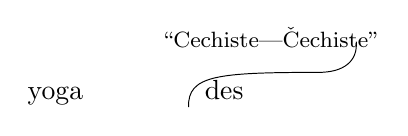
\begin{tikzpicture}[baseline=(yogab.base),x=1cm,y=1cm]
\node[anchor=base west,inner sep=0pt] (yogab) at (0,0) {yoga};
\node[anchor=base west,inner sep=0pt] at (2.25,0) {des};
\node[anchor=base west,inner sep=0pt,font=\footnotesize] at (1.70,.66) {\inserted{``\unsure{Cechiste|\v{C}echiste}''}};
\draw[line width=.35pt] (2.05,-.10) .. controls (2.04,.30) and (2.40,.34) .. (3.70,.34)
 .. controls (4.02,.34) and (4.20,.48) .. (4.18,.73);
\end{tikzpicture} recouvrements \unsure{et de} leurs nerfs, et le raffinement de ce y.g. suggéré par Cartier (pour les espaces topologiques non paracompacts). Voici les conditions qui me viennent à l'esprit:

\uline{Hyp 1} Les objets $U_\alpha$ ($\alpha\in\mathrm{Ob}\,A$) recouvrent l'\unsure{objet|objt} final $e_{\mathcal X}$ de $\mathcal X$.

\deleted{\uline{Hyp 1'} Pour tout $\alpha_0\in\mathrm{Ob}\,A$, le foncteur induit $A/\alpha_0\longrightarrow\mathcal X/U_{\alpha_0}$ satisfait à Hyp 1, i.e. l'ens. des flèches $U_\alpha\longrightarrow U_{\alpha_0}$, associé aux flèches $\alpha\longrightarrow\alpha_0$ de but $\alpha_0$ dans $A$,}
\margin{Est satisfait tautologiquement!}
\margin{10}
